
\documentclass{article}

\usepackage[dvipsone]{graphicx}
\usepackage{afterpage}

%\setlength{\topmargin}{0mm}
\setlength{\topmargin}{-20mm}
\setlength{\oddsidemargin}{5mm}
\setlength{\textwidth}{160mm}
\setlength{\textheight}{240mm}

%\pagestyle{empty}

\begin{document}

\noindent
{\Large \bf Elevation Angle Determination} \\[5mm]

\noindent
Simon G.~Shepherd \hfill \today \\[5mm]

\noindent
{\large \bf Definitions} \\

\noindent
$\phi_0$ -- beam azimuth at 0$^\circ$ elevation angle \\
$\phi$ -- beam azimuth at non-zero elevation angle \\
$\theta$ -- elevation angle \\
$\hat{n}$ -- normal unit vector in the direction of the beam \\
$X$ -- offset of interferometer array in $\hat{x}$ direction \\
$Y$ -- offset of interferometer array in $\hat{y}$ direction \\
$Z$ -- offset of interferometer array in $\hat{z}$ direction \\
$f$ -- tranmission frequency \\
$d$ -- distance between phase fronts in planes passing through arrays\\[5mm]

\noindent
{\large \bf Background} \\
%\section{Background}

\noindent
The elevation angle is a measurement that can be made with a SuperDARN
radar that has both a main and interferometer array. A calibration procedure
must be followed to determine the signal delays through each path from
the respective array to the digitizer. This calibration procedure is
describe in a separate document. In addition, the software at the radar must
be configured to compute and save cross-correlation functions (XCFs). \\

\noindent
We currently have a procedure to compute the elevation angle that is located
in {\tt elevation.c}. It was written by Kile Baker and possibly Simon Wing,
and modified somewhat by Robin Barnes. Comments in the code are not sufficient
to fully understand the code. It would be useful to identify a document that
describes this code. Note that this code appears to work well for simple
situations, i.e., interferometer array offsets that are in front of or behind
the main array. However, the results do not appear consistent for more
complicated offsets, i.e., those in the vertical direction or along the
direction of the main array. Note that there is a special program called
{\tt elev\_goose.c} that is used for the Goose Bay radar. This program is
specific to the geometry of this radar and gets stuck in an infinite loop
when used on other geometries. \\

\noindent
I believe there is a simpler and more general method to determine the angle
of arrival of signals from a SuperDARN radar. The basic idea is that it is
possible to determine the distance between two parallel planes, one passing
through the center of the main array and the other passing through the center
of the inteferometer array. The separation between these two planes
is a function of the beam azimuth ($\phi$), the elevation angle ($\theta$),
the tranmission frequency ($f$) and the physical separation between the
centers of the antennas ($X$,$Y$,$Z$). The separation between these two planes
introduces a phase difference in the signals. By equating this difference
(including also a constant phase offset due to the electronics and cables)
to the observed phase delay in the two signals, a quadratic equation can be
solved for the elevation angle. This technique is described below. \\

\noindent
{\large \bf A More General Technique} \\

\noindent
To solve this quadratic equation it is first necessary to write the equations
for the two planes. The normal unit vector of the planes is in the direction
the signals are coming from and is given by:

\begin{equation}
\hat{n} = \left( \cos \theta \sin \phi \right) \hat{x} +
					\left( \cos \theta \cos \phi \right) \hat{y} +
					\left( \sin \theta \right) \hat{z} \label{eq:norm}
\end{equation}

\noindent
or introducing $A \equiv \cos \theta \sin \phi$,
$B \equiv \cos \theta \cos \phi$ and $C \equiv \sin \theta$:

\begin{equation}
\hat{n} = A \hat{x} + B \hat{y} + C \hat{z}
\end{equation}

\noindent
Using the convention that the center of the main array is located at the
origin and the center of the interferometer array is located at position
$(X,Y,Z)$ we can write equations for planes passing through these locations
and both oriented normal to $\hat{n}$.

\begin{eqnarray}
\mathbf{main:} & Ax + By + Cz & = 0 \equiv d_{main} \\
\mathbf{int.:} & A(x-X) + B(y-Y) + C(z-Z) & = 0 \\
& Ax + By + Cz & = AX + BY + CZ \equiv d_{int}
\end{eqnarray}

\noindent
Note that this convention is the standard that is used in {\tt hardware.dat}
files. The distance between these two planes is given by:

\begin{eqnarray}
d & = & \frac{d_{int} - d_{main}}{A^2 + B^2 + C^2} \\
  & = & AX + BY + CZ \label{eq:d} \\
  & = & \left( \cos \theta \sin \phi \right) X +
          \left( \cos \theta \cos \phi \right) Y +
          \left( \sin \theta \right) Z \label{eq:dist}
\end{eqnarray}
since $\hat{n}$ is a unit vector the denominator is unity. \\

\noindent
Note that the beam azimuth ($\phi$ is actually a function of elevation
angle ($\theta$). There is something called the {\it coning angle} in
which the phases of the antennas interfere along a cone around the axis
of the array. [{\bf I don't really understand this bit.}] The functional
form of this coning angle is given by:

\begin{equation}
\sin \phi = \frac{\sin \phi_0}{\cos \theta}
\end{equation}

\noindent
Equation \ref{eq:norm} can be modified by using the coning angle equation
and

\begin{equation}
\cos \phi = \left(1 - \sin^2 \phi \right)^{\frac{1}{2}} =
\left(\cos^2 \theta - \sin^2 \phi_0 \right)^{\frac{1}{2}} / \cos \theta
\end{equation}

\noindent
giving

\begin{equation}
\hat{n} = \sin \phi_0 \hat{x} +
          \left(\cos^2 \theta - \sin^2 \phi_0 \right)^{\frac{1}{2}} \hat{y} +
          \sin \theta \hat{z}
\end{equation}

\noindent
and modifying $A \equiv \sin \phi_0$,
$B \equiv \left(\cos^2 \theta - \sin^2 \phi_0 \right)^{\frac{1}{2}}$ and 
$C \equiv \sin \theta$ so that equation \ref{eq:d} is still valid and
equation \ref{eq:dist} becomes:

\begin{eqnarray}
d & = & AX + BY + CZ \\
  & = & \left( \sin \phi_0 \right) X +
        \left(\cos^2 \theta - \sin^2 \phi_0 \right)^{\frac{1}{2}} Y +
          \left( \cos \theta \cos \phi \right) Y +
          \left( \sin \theta \right) Z \label{eq:the_dist}
\end{eqnarray}

\noindent
The delay to the signal caused by the offset between the arrays is given by:

\begin{equation}
\phi_{geo} = k d %\hspace{1cm} \mathrm{[radians]}
\end{equation}

\noindent
where $k = 2 \pi / \lambda = 2 \pi c / f$ is the wavenumber, $c$ is the speed
of light and $f$ is the transmission frequency. Note that $\phi_{geo}$ is a
nonlinear function of the elevation angle, $\theta$, and is the phase delay
due to geometry; array separation and look-direction. \\

\noindent
There is an additional delay in SuperDARN systems that is introduced by
differences in the paths that signal make from the main array and the
interferometer array. This delay is largely due to differences in cable
lengths to the antenna arrays, but can also be due to differences in the
electrical paths in the electronics. As part of a proper calibration the
time difference between the two paths (from antenna to digitizer) is measured
and entered in the {\tt hardware.dat} file as the parameter $t_{diff}$. This
number is typically a few hundred nanoseconds and is listed in the file as a
decimal number of microseconds.

\noindent
Using this measured time delay the phase delay associated with $t_{diff}$ is
given by:

\begin{equation}
\phi_{path} = 2 \pi f t_{diff}
\end{equation}

\noindent
Note that these delays are in the opposite sense. For example, in the MSI
radars the interferometer arrays is behind the main array, so $X = Z = 0$
and $Y < 0$ so that $\phi_{geo} < 0$ for any beam direction coming from in
front of the arrays. In this situation signals arrive at the main array before
the interferomter array. On the other hand, the interferometer cables are
much shorter than the main array cables (350 ft compared to 650 ft) and
$t_{diff} < 0$, by convention. In this case the signals arrive at the
interferometer array because the electrical path is short. The total delay
is then given by:

\begin{equation}
\phi_{total} = \phi_{geo} - \phi_{path} \label{eq:total} \\[5mm]
\end{equation}

\noindent
In the SuperDARN system the phase difference between the main and
interferometer array is calculated from the auto-correlation (ACF) and
cross-correlation (XCF) functions. One complication is that the phase delay
obtained from the ACF and XCF is only the residual phase and is between
$-\pi$ and $\pi$. It is likely that the observed delay is actually several
multiples of $2\pi$, however, it is not possible to definitively determine
the actual phase delay from the ACF and XCF measurements alone. The
implications of this ambiguity in the observed phase difference is two-fold.
First, there is an inherent limitation in the maximum elevation angle that
can be uniquely determined. This maximum elevation angle depends on the
separation between the arrays and the beam direction ($\phi_0$). \\

\begin{figure}[tb]
\includegraphics[scale=.9]{80m-2pi.ps}
\caption{Maximum elevation angle before a $2\pi$ ambiguity in the observed
phase is introduced. The example shown is for the MSI Oregon radar
configuration in which the interferometer arrays are offset behind the main
arrays by 80 m. No other offsets are present.}
\label{fig:2pi}
\end{figure}

\noindent
Figure \ref{fig:2pi} shows the maximum elevation angle for the MSI Oregon
radars in which the interferometer arrays are offset behind their respective
main arrays by a distance of 80 m, i.e., ($X$,$Y$,$Z$) = (0,-80,0). As shown,
the maximum elevation angle decreases from a maximum value of $\sim$60$^\circ$,
for a transmission frequency of 8.0 MHz and looking normal to the array, for
both higher frequencies and for beams looking off the boresight direction. \\

\noindent
The second impact is that the residual phase must shifted by the appropriate
number of 2$\pi$ factors in order to match the delays that are introduced
by the other factors; geometry and electrical path. The need for this shifting
introduces the possibilty that the elevation angle determined can be
significantly from the actual elevation angle. \\

\noindent
Once the appropriate number of 2$\pi$ factors have been added to the
observed residual phase, the resulting phase difference ($\phi_{obs}$) is
used to determine an equation that depends on the elevation angle. Equating
the observed and expected phase delays gives:

\begin{equation}
\phi_{total} = \phi_{geo} - \phi_{path} = \phi_{obs}
\end{equation}

\noindent
which can be written as:

\begin{eqnarray}
\phi_{obs} + \phi_{path} & = & \phi_{geo} \\
                         & = & k d \\
                         & = & k \left[
                                 \sin \phi_0 X +
                                 \left( \cos^2\theta - 
																				\sin^2\phi_0 \right)^\frac{1}{2} Y +
                                 \sin \theta Z
                                 \right]
\end{eqnarray}

\noindent
Rearranging and using the identity $\sin^2 \theta + \cos^2 \theta = 1$:

\begin{equation}
\left[1 - \sin^2\theta - \sin^2\phi_0 \right] Y^2 =
	\left[ \frac{\phi_{obs} + \phi_{path}}{k} - \sin \phi_0 X - \sin \theta Z
	\right]^2
\end{equation}

\noindent
and simplifying using the following factors:

\begin{eqnarray}
D & \equiv & 1 - \sin^2 \phi_0 \\
E & \equiv & \frac{\phi_{obs} + \phi_{path}}{k} - \sin \phi_0 X
\end{eqnarray}

\noindent
We can write this equation as:

\begin{eqnarray}
\left[ D - \sin^2 \theta \right] Y^2 & = & \left[ E - \sin \theta Z \right]^2\\
& = & E^2 - 2 E Z \sin \theta + \sin^2 \theta Z^2
\end{eqnarray}

\noindent
and finally as:

\begin{equation}
\left( Z^2 + Y^2 \right) \sin^2 \theta - 2 E Z \sin \theta +
	\left( E^2 - D Y^2 \right) = 0 \label{eq:quad}
\end{equation}


\noindent
Equation \ref{eq:quad} is a quadratic equation in $\sin \theta$ and can be
easily solved:

\begin{eqnarray}
\sin \theta & = & \frac{
	EZ \pm \left[ E^2 Z^2 - \left(Z^2 +Y^2\right)\left(E^2 - DY^2\right)
			\right]^\frac{1}{2}}
	{Z^2 + Y^2} \\
& = & \frac{EZ \pm \left|Y\right| \left[ D \left(Z^2 + Y^2\right) - E^2
		\right]^\frac{1}{2}}{Z^2 + Y^2} \label{eq:sin_theta}
\end{eqnarray}

\noindent
The solution to equation \ref{eq:sin_theta} gives the elevation angle $\theta$
in terms of known quantities.

\begin{figure}[tb]
\includegraphics[scale=.8]{angle_eg.ps}
\caption{Dark blue curves show the phase delay introduced by the separation
of the main and interferometer arrays for two different beam directions. The
intersection of these curves with the observed delay, indicated by the
hozrizonal solid red line, gives the elevation angle from equation
\ref{eq:sin_theta}. Horizontal vertical dotted lines show the good agreement
with the existing methods currently used to determine elevation angles.}
\label{fig:elev}
\end{figure}

\noindent
Figure \ref{fig:elev} shows an example of solving equation \ref{eq:sin_theta}
for two different beams (12 and 21) with the MSI Oregon geometry. The
dark blue curves are the total delay $\phi_{total}$ from equation
\ref{eq:total} for the two different beams. Note that for simplicity
$t_{diff}$ is assumed to be zero so that $\phi_{path}$ is also zero. A
non-zero value would simply shift the blue curves vertically by the
appropriate constant phase delay. \\

\noindent
An additional curve is shown in a lighter shade of blue. This is the total
delay ignoring the coning angle equation and is shown for context only. Note
that for beams that are close to the boresight (e.g., beam 12 in a 24 beam
array) the two curves are nearly identical. \\

\noindent
The horizontal solid red line is the observed residual phase delay adjusted
with the appropriate number of 2$\pi$ factors. The intersection of the red
and blue curves gives the elevation angle $\theta$ from equation
\ref{eq:sin_theta}. Vertical dotted lines extending downward from the
horizontal red line show this solution for the two beams (and the uncorrected
lighter blue curves). The solution given by our current algorithm ({\tt
elevation.c}) is indicated by vertical dotted lines that extend upward from the
horizontal red line and show very good agreement with our computed values.\\

\begin{figure}[tb]
\includegraphics[scale=.8]{beam12_eg.ps}
\caption{Elevation angles for observed residual phase delays ranging from
-$\pi$ to $\pi$. The solid dark blue curve shows the result of equation
\ref{eq:sin_theta}. The purple curve is for reference only and shows the
result if the coning angle equation is not used. A dotted orange curve shows
the result of our current algorithm and lies on top of the dark blue curve.
The lower figure shows the difference between the new method and the current
technique.}
\label{fig:beam12}
\end{figure}

\begin{figure}[tb]
\includegraphics[scale=.8]{beam21_eg.ps}
\caption{The same format as Figure \ref{fig:beam12} but for beam 21.}
\label{fig:beam21}
\end{figure}

\noindent
Figures \ref{fig:beam12} and \ref{fig:beam21} show examples of the agreement
between the two techniques for two different beams; 12 and 21. The errors
between the two techniques are around 10$^{-5}$ degrees. Note the shift in
elevation angle around -2 radians. \\

\noindent
While the agreement is good for the simplest situation (and it should be
noted that most SuperDARN radars fall into this category) there are difference
between the two techniques for more complicated array separations, i.e.,
those with offsets in more than just the $\hat{y}$ direction. \\

\begin{figure}[tb]
\includegraphics[scale=.8]{10MHz_X.ps}
\caption{Elevation angles for a range of offsets in the $\hat{x}$ direction.
Blue curves show the result for various beams using equation
\ref{eq:sin_theta} while the dotted red lines show the result using the
existing algorithm. The two solutions agree for zero offset in the $\hat{x}$
direction, but differ increasingly for larger offsets.}
\label{fig:dX}
\end{figure}

\noindent
Figure \ref{fig:dX} shows the elevation angles calculated using equation
\ref{eq:sin_theta} in solid blue and the current algorithm in dotted red
for a range of offsets in the $\hat{x}$ direction, i.e., along the direction
of the arrays. Note that the Goose Bay radar and a few others falls into this
category, but the offset in the $\hat{x}$ direction is small compared to the
offset in the $\hat{y}$ direction. \\

\noindent
Note that the result using our current technique cannot be correct. While
there is some dependence of the elevation angle on the amount of offset in
the $\hat{x}$ direction, it is the same for symmetric beams on either side
of the boresight. This result is clearly not correct as the distance between
planes for beams oriented toward the direction of the offset must be smaller
than in the direction of the boresight. The opposite must be true for beams
oriented away from the direction of the offest. The blue curves show this
behavior. \\

\begin{figure}[tb]
\includegraphics[scale=.8]{10MHz_Z+.ps}
\caption{The same format as figure \ref{fig:dX} but for offsets in the
$\hat{z}$ direction. Again, the two solution agree for zero offset in the
$\hat{z}$ direction, but differ substantially for larger offsets.}
\label{fig:dZ}
\end{figure}

\noindent
Figure \ref{fig:dZ} shows that the elevation angles computed using the
two techniques is more complicated for offsets in the $\hat{z}$ direction.
Here there is good agreement for some offsets, but there are significant
jumps in the elevation angles computed using the current algorithm (dotted
red curves) and negative angles that are reported for positive offsets.
Note that in practice offsets in the $\hat{z}$ direction are limited to
$\pm$5--10 m, but there are still measureable difference in this limited
range. \\


\noindent
{\large \bf Conclusions} \\

\noindent
The existing technique works well and gives the expected results for the
simple situation in which the interferometer array is offset only in the
boresight direction ($\hat{y}$). For more complicated offsets the results
obtained from our current technique are incorrect. A better, more intuitive
and more general method for determining the elevation angle has been descibed.
Note that more testing is necessary to refine the algorithm so that it can
deal with the following situations:

\begin{itemize}
\item non-zero $t_{diff}$ -- testing is necessary to make sure that the
appropriate number of 2$\pi$ factors are always used.
\item $\phi_{diff}$ -- this is parameter that was introduced to account for
errors in connecting the main and interferometer cables. It has not been
incorporated in the analysis, but should be.
\item offsets -- more testing for offsets in the $\hat{x}$ and $\hat{z}$
directions is needed to be sure that the jumps in elevation angle are real
and that the separation between the planes in 3D is consistent with the
computed elevation angle.
\item coning angle -- a more complete description of this phenomenon is
needed for this document.
\end{itemize}

\end{document}

